% Compile with pdflatex synrxn-workflow-1.5.0.tex.
% Family labels and task count follow the SynRXN 1.5.0 catalog.
\documentclass[tikz,border=3pt]{standalone}
\usepackage[T1]{fontenc}
\usepackage{lmodern}
\usepackage{fontawesome5}
\usetikzlibrary{arrows.meta}

\definecolor{Ink}{HTML}{18324F}
\definecolor{Muted}{HTML}{4F647A}
\definecolor{Navy}{HTML}{153862}
\definecolor{Blue}{HTML}{285F91}
\definecolor{BlueEdge}{HTML}{C1D3E5}
\definecolor{BlueWash}{HTML}{F0F5FA}
\definecolor{Teal}{HTML}{006A6B}
\definecolor{TealInk}{HTML}{005657}
\definecolor{TealEdge}{HTML}{A0D4D0}
\definecolor{TealWash}{HTML}{EDF8F7}
\definecolor{Hold}{HTML}{9D4647}
\definecolor{HoldWash}{HTML}{FCF3F2}

\renewcommand{\familydefault}{\sfdefault}
\tikzset{
  panel title/.style={font=\bfseries\fontsize{10.4}{12}\selectfont,
    text=white, align=center, inner sep=0pt},
  step title/.style={font=\bfseries\fontsize{10.1}{11.5}\selectfont,
    text=Ink, anchor=west, inner sep=0pt},
  small text/.style={font=\fontsize{8.4}{10}\selectfont,
    text=Muted, inner sep=0pt, align=center},
  flow arrow/.style={-{Stealth[length=3.0mm,width=2.4mm]},
    line width=1.3pt, draw=Teal},
}

% x, y, width, height, accent, fill, title
\newcommand{\workflowpanel}[7]{%
  \begin{scope}[shift={(#1,#2)}]
    \fill[#6,rounded corners=2mm] (0,0) rectangle (#3,-#4);
    \begin{scope}
      \clip[rounded corners=2mm] (0,0) rectangle (#3,-#4);
      \fill[#5] (0,0) rectangle (#3,-0.86);
    \end{scope}
    \draw[#5,rounded corners=2mm,line width=0.75pt] (0,0) rectangle (#3,-#4);
    \node[panel title] at ({#3/2},-0.43) {#7};
  \end{scope}%
}

% Top edge, step number, icon, heading
\newcommand{\curationstep}[4]{%
  \begin{scope}[shift={(4.18,#1)}]
    \filldraw[fill=white,draw=BlueEdge,rounded corners=1.4mm]
      (0,0) rectangle (5.74,-1.18);
    \node[circle,fill=Navy,text=white,font=\bfseries\small,
      inner sep=0pt,minimum size=4.7mm] at (0.37,-0.59) {#2};
    \node[rounded corners=1.15mm,fill=BlueWash,text=Blue,
      font=\fontsize{11}{11}\selectfont,minimum width=6mm,minimum height=6mm]
      at (1.03,-0.59) {\faIcon{#3}};
    \node[step title] at (1.52,-0.59) {#4};
  \end{scope}%
}

% x, y, icon, family label
\newcommand{\familycard}[4]{%
  \begin{scope}[shift={(#1,#2)}]
    \filldraw[fill=white,draw=TealEdge,rounded corners=1.35mm]
      (0,0) rectangle (3.52,-0.94);
    \node[rounded corners=1mm,fill=TealWash,text=Teal,
      font=\fontsize{9.4}{9.4}\selectfont,minimum width=5mm,minimum height=5mm]
      at (0.37,-0.47) {\faIcon{#3}};
    \node[anchor=west,align=left,font=\bfseries\fontsize{8.5}{9.7}\selectfont,
      text=TealInk,inner sep=0pt,text width=2.75cm] at (0.74,-0.47) {#4};
  \end{scope}%
}

\begin{document}
\begin{tikzpicture}[x=1cm,y=1cm,line cap=round,line join=round]
  \fill[white] (0,0) rectangle (22.5,-10.2);

  \workflowpanel{0.23}{-1.66}{3.20}{5.68}{Blue}{BlueWash}{Reaction data\\sources}
  \workflowpanel{3.95}{-0.42}{6.20}{8.25}{Navy}{BlueWash}{Data preparation}
  \workflowpanel{10.73}{-2.42}{3.14}{4.31}{Teal}{TealWash}{SynRXN 1.5.0}
  \workflowpanel{14.46}{-0.42}{7.77}{8.25}{Teal}{TealWash}{Evaluation}

  \draw[flow arrow,draw=Navy] (3.44,-4.65) -- (3.94,-4.65);
  \draw[flow arrow] (10.16,-4.65) -- (10.72,-4.65);
  \draw[flow arrow] (13.88,-4.65) -- (14.45,-4.65);

  % Source collections and reaction glyph.
  \begin{scope}[shift={(0.64,-3.16)}]
    \draw[Blue,line width=1.05pt] (0,0.14)--(0.28,-0.06)--(0.61,0.02)--(0.78,0.25)
      (0.28,-0.06)--(0.1,-0.31);
    \foreach \x/\y in {0/0.14,0.28/-0.06,0.61/0.02,0.78/0.25,0.1/-0.31}
      \fill[Blue] (\x,\y) circle (0.048);
    \draw[-{Stealth[length=1.9mm]},Teal,line width=1pt] (0.93,-0.02)--(1.35,-0.02);
    \draw[Teal,line width=1.05pt]
      (1.53,-0.19)--(1.77,0.06)--(2.07,-0.03)--(2.29,0.19)
      (2.07,-0.03)--(2.3,-0.29);
    \foreach \x/\y in {1.53/-0.19,1.77/0.06,2.07/-0.03,2.29/0.19,2.3/-0.29}
      \fill[Teal] (\x,\y) circle (0.048);
  \end{scope}
  \draw[BlueEdge] (0.54,-3.68) -- (3.12,-3.68);
  \foreach \y/\entry in {
    -4.12/{Patents \&\\literature},
    -4.78/{Databases},
    -5.40/{Experiments},
    -6.03/{Curated\\references},
    -6.73/{Simulations}} {
    \fill[Blue,rounded corners=0.2mm] (0.55,{\y+0.046}) rectangle (0.64,{\y-0.046});
    \node[anchor=west,font=\fontsize{8.2}{9.3}\selectfont,text=Ink,inner sep=0pt,
      align=left,text width=2.43cm] at (0.79,\y) {\entry};
  }

  \curationstep{-1.56}{1}{link}{Pin source versions}
  \curationstep{-2.94}{2}{check-circle}{Validate records}
  \curationstep{-4.32}{3}{table}{Prepare tables}
  \curationstep{-5.70}{4}{project-diagram}{Group related records}
  \curationstep{-7.08}{5}{tasks}{Set targets and metrics}

  \draw[-{Stealth[length=2mm]},Hold,dashed,line width=0.8pt]
    (7.05,-8.68) -- (7.05,-9.00);
  \filldraw[fill=HoldWash,draw=Hold,dashed,rounded corners=1.2mm]
    (4.39,-9.02) rectangle (9.71,-9.94);
  \node[text=Hold,font=\fontsize{10}{10}\selectfont] at (4.80,-9.48) {\faIcon{clipboard-list}};
  \node[step title,text=Hold] at (5.17,-9.48) {Held or excluded records};

  \node[text=Teal,font=\fontsize{34}{34}\selectfont] at (12.30,-4.45) {\faIcon{database}};
  \node[font=\bfseries\fontsize{9.0}{10.4}\selectfont,text=TealInk]
    at (12.30,-5.73) {Data release};

  \node[small text,text=TealInk,font=\bfseries\fontsize{8.8}{10.5}\selectfont]
    at (18.345,-1.65) {12 families \textperiodcentered{} 40 tasks};
  \familycard{14.70}{-2.03}{share-alt}{Mechanisms\\\& networks}
  \familycard{18.47}{-2.03}{wave-square}{Physics \& kinetics}
  \familycard{14.70}{-3.10}{exchange-alt}{Single-step\\transformations}
  \familycard{18.47}{-3.10}{search}{Representation\\\& search}
  \familycard{14.70}{-4.17}{vials}{Selectivity\\\& mixtures}
  \familycard{18.47}{-4.17}{chart-line}{Outcomes\\\& feasibility}
  \familycard{14.70}{-5.24}{sliders-h}{Conditions\\\& procedures}
  \familycard{18.47}{-5.24}{chart-bar}{Analysis\\\& monitoring}
  \familycard{14.70}{-6.31}{file-alt}{Data acquisition\\\& curation}
  \familycard{18.47}{-6.31}{draw-polygon}{Components\\\& reactivity}
  \familycard{14.70}{-7.38}{industry}{Process engineering}
  \familycard{18.47}{-7.38}{dna}{Biocatalysis\\\& enzyme function}
\end{tikzpicture}
\end{document}
